\documentclass[]{scrartcl}

\usepackage{geometry}
\usepackage{graphicx}
\usepackage{listings}
\usepackage{amsmath}
\usepackage{mathtools}
\usepackage{hyperref}
\usepackage{mdwlist}
\usepackage{afterpage}
%\usepackage{enumitem}
\usepackage{pdfpages}
\usepackage{textcomp}
\usepackage{amsmath}
\usepackage{multicol}
\usepackage[english]{babel}
\usepackage{siunitx}
\usepackage{subfigure}


\usepackage[utf8]{inputenc}

\usepackage{fixme} 
\fxsetup{
     status=final,					% change to draft or final in the end
     author=GS,                                            % name to prepend before all annotations
     layout=margin,
     theme=color
}
\usepackage[autostyle]{csquotes}
\usepackage[style=authoryear,backend=bibtex,bibencoding=utf8,mincitenames=2,maxcitenames=3, hyperref=true,url=false,eprint=false]{biblatex}
\addbibresource[]{npliterature.bib}

%opening
\title{Nanopore Results % \\ \Large (DRAFT)
}
\author{Gregor Sturm}

\begin{document}

\maketitle

\begin{abstract}
\begin{description}
\item This report is a short outline of my work on Nanopore Basecalling from 2015-06 until 2016-01. It is the outcome of a student project at the Institute of Bioinformatics and Systems Biology (IBIS) of the Helmholtz-Zentrum München. Here, I presents the major results of this project. 
\item [Availability] Analysis are available as iPython-Notebooks in the github repository \url{https://github.com/grst/nanopore}. The code of the novel python basecaller is available in the repository \url{https://github.com/grst/nanopore\_pkg}. 
\item [Contact] gregor.sturm@cs.tum.edu
\end{description}

\end{abstract}

\section{Introduction to Nanopore Basecalling}
%Nanopore-Sequencing is a recent 'third-generation' sequencing approach. Unlike previous state-of-the-art sequencing methods, such as Illumina, which are all based on a sequencing-by-synthesis approach, Nanopore sequencing is a promising technology which determines the sequence of a DNA strand exploiting the pysical properties of the different nucleotides. 
%
%The idea of nanopore sequencing is not new and is under investigation for decades. Recently, Oxford Nanoporetech presented the MinION sequencing device. A sequencer not larger than a customary USB Hard drive. It may be plugged into a Standard-PC via USB 3.0 and connects with the company's "Metrichor" analysis cloud which performs the analysis of the generated data. 
%
%The functioning and usage of the device is fairly straight-forward: After DNA purification and preparation, the sample is put on a flow-cell. Every flow-cell consists of an "upper" and a "lower" chamber and is separated into 512 departments, each of which is equipped with a protein-pore connecting the two chambers. After a voltage is applied on the membrane, the negative charge of the DNA moleclues is exploited to pull the molecules through the pore from the upper into the lower chamber. It is assumed, that six nucleotides are in the pore at the same time. Depending on the exact sequence of these six nucleotides, more or less Kations can pass the pore in the opposite direction, which can be measured as the electric current of the pore. Translating these signals into the corresponding nucleotide sequence is data-intensive machine learning task which is commonly solved using Hidden Markov Models (HMMs). According to expert opinions from the MinION community platform "The sensors are better than the chemistry and the chemistry is better than the software at the moment", thus the software being the limiting factor of the quality of nanopore reads. 
%
%Unfortunately the Basecalling-Pipeline used by Oxford Nanopore is under closed source and works as a blackbox. Thus, it's detailed functioning is not known, but the major steps can be derived from data and log files generated by this software. In this project, we developed an open-source baseline basecalling algorithm, which can be taken as a basis for future projects aiming at matching and exceeding the performance of the Metrichor basecaller. Moreover, we present an extended context analysis of signals and point towards improved alignment techniques. 

% explain functioning. 
The MinION by Oxford Nanopore Technologies (ONT) is a 'fourth-generation' sequencing device not larger than a portable hard drive. The device is connected with a customary PC and interacts with the Company's \textit{Metrichor} cloud for \textit{basecalling}, i.e. translation of the raw signal into the DNA sequence (\cite{Feng2015}). 

The functioning and usage of the device is fairly straight-forward: After DNA purification and preparation, the sample is put on a flow-cell. Every flow-cell consists of an "upper" and a "lower" chamber and is separated into 512 compartments, each of which is equipped with a protein pore connecting the two chambers. After a voltage is applied on the membrane, the negative charge of the DNA molecules is exploited to pull the them through the pore from the upper into the lower chamber. It is assumed, that six nucleotides are in the pore at the same time. Depending on the exact sequence of these six nucleotides, more or less cations can pass the pore in the opposite direction, which can be measured as the electric current.\footnote{Information collated from various posts in the Nanoporetech wiki and \cite{Feng2015}} 

Translating these signals into the corresponding nucleotide sequence is data-intensive machine learning task which is commonly solved using Hidden Markov Models (HMMs) (\cite{Timp2012a}). Unfortunately, the Metrichor basecaller is closed source and works as a black box. Uploading data to the analysis cloud is not an option when (i) dealing with critical patient data and (ii) sequencing at places with an unstable Internet connection. Moreover, an open source basecaller would be a valuable contribution to the field, as it can easily be applied and improved by other research groups.

I address this with the python package \texttt{npcaller}, an open source implementation of a HMM-based basecaller for the MinION. 

All data used in this work is based on the SQK-MAP006 sequencing kit. ONT has recently announced a new flow cell and basecaller (see section \ref{sec:future}). It is likely that \texttt{npcaller} will not work with the future version of MinION. 

\section{Overview over the ONT Basecalling Pipeline}
\subsection{File formats}
All data generated during the MinION basecalling pipeline is stored in \texttt{fast5} files, which are built upon the \texttt{HDF5}\footnote{\url{https://www.hdfgroup.org/HDF5/}} data storage format. \texttt{HDF5} contains a directory-like hierarchical structure. Every directory can have attributes and/or contain data-tables. The HDF group provides software for viewing and manipulating \texttt{HDF5}-files\footnote{\url{https://www.hdfgroup.org/products/java/release/download.html}}. Moreover, there is the python library \texttt{h5py} for programmatic interaction with the contents\footnote{\url{http://www.h5py.org/}}

%\subsection{Types of \texttt{fast5}-files}
%%%raw files, unprocessed / processed fast5 files. 
%%
%%% 5mer and 6mer formats
%%
%%% future directions

\subsection{The Pipeline}
The Metrichor Basecalling Pipeline consists of the following major steps\footnote{Reverse engineering of \textit{Metrichor} data files and posts in the internal wiki}. Check figure \ref{fig:squiggle} for an illustration of the data. 

\begin{enumerate}
\item \textbf{Raw data.} Sensors measure the electric current over the pore at a fixed sample-rate, which is \SI{3000}{\hertz} for SQK-MAP006.
\item \textbf{Event calling.} This step serves for reducing the amount of data. Consecutive samples with similar mean are combined into one \textit{event} or \textit{squiggle}. An event is a tuple \texttt{(start\_time, length, mean, stdv)}. The resulting set of squiggles is often referred to as \textit{Squiggle space}. 
\item \textbf{(1D) Base calling.} The events are converted to a nucleotide sequence using a HMM (\cite{Timp2012a}). Other than in the paper, by now the MinION uses 6-mers. The HMM has therefore $2^6 = 4096$ states. 
\item \textbf{2D base calling.} To improve accuracy, the MinION supports 2D basecalling. Here, forward and reverse strand of the DNA are ligated together using a hairpin adapter. Like that, the same sequence is read twice, once in sense and once in antisense direction. In 2D base calling, the two 1D reads are aligned and uncertainities resolved.   
\end{enumerate}




\begin{figure}[htbp]
\centering
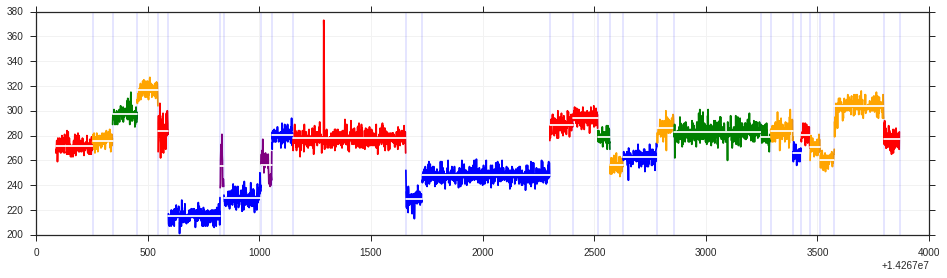
\includegraphics[width=\linewidth]{figures/squiggle.png}
\caption{Exemplary raw Data divided into events. The measured current (y) is plotted against the time (x). Each section separated by two vertical lines represents one \textit{event}, consisting of many individual current samples measured by the sensor. The white, horizontal lines represent the mean of the respective event. }
\label{fig:squiggle}
\end{figure}



\section{The Basecalling Package}
I developed the python package \texttt{npcaller} which provides alternative basecalling for the MinION. The software consists of three major parts:

\begin{enumerate}
\item Model generation
\item Basecalling
\item Validation.
\end{enumerate}

The software depends on the python packages \texttt{h5py, ghmm, numpy, pandas} and \texttt{pysam} which are all available trough the python package index\footnote{\url{https://pypi.python.org/pypi}} and can be installed using \texttt{pip install}. Additionally, the package uses the following command line software, which has to be available on the machine: 
\begin{itemize}
\item \textbf{graphmap} (\cite{Sovic2015GRAPHMAP}) is a novel, specialized aligner for long, error-prone reads as they are generated by nanopore sequencing devices and is available through github\footnote{\url{https://github.com/isovic/graphmap}}.
\item \textbf{samtools} (\cite{Li2009SAMTOOLS}) is a commonly used tool for handling alignment files. It is available on \url{http://samtools.sourceforge.net/}
\item \textbf{poretools} (\cite{Loman2014PORETOOLS})  is a toolkit for analyzing nanopore sequencing data. It is available on github\footnote{\url{https://github.com/arq5x/poretools}} or through \texttt{pip install poretools}. Poretools is only required for the validation part of the software. 
\end{itemize}

\subsection{Documentation}
This documentation aims at explaining what's going on under the hood. For description of the program calls, see the help pages of the scripts themselves. 
 
\subsubsection{Model generation}
In the first step, one needs to retrieve the parameters (i.e.\ mean and standard deviation for each kmer) for the HMM. Template and complement DNA strands show a different base calling behaviour, therefore two models are generated. The package provides two scripts for the model generation: 

\begin{itemize}
\item \texttt{model\_from\_fast5.py}: The parameters used by \textit{Metrichor} are saved as metadata in the fast5-files. This script extracts this data and saves it as a model. 
\item \texttt{model\_from\_alignment.py}: This script computes the parameters by aligning a set of basecalled (e.g.\ by \textit{Metrichor}) fast5-files to a reference genome. For every $\mathrm{kmer} \in \{\mathrm{AAAAAA}, \dots, \mathrm{TTTTTT}\}$, the mean and standard deviation of the current among all occurrences in the reference genome is calculated. As this script involves the aligning of many reads, it is quite computationally expensive and provides the option to run multithreaded. 
\end{itemize}

\subsubsection{Basecalling}
\texttt{basecall.py} takes a list of (uncalled) fast5 files and model files as input and writes the resulting nucleotide sequence to a fasta file. Template and complement model files can be specified separately. If only one of them is specified, only only the corresponding sequence will be called. As this process is CPU-intensive, the script provides the option to run multithreaded. 

\subsubsection{Validation}
\texttt{validate.py} comes with four sub-programmes:
\begin{itemize}
\item \texttt{randomize} takes a fasta file as input and mutates all nucleotides assuming a uniform distribution. The original sequence lengths are kept. This is useful to compare the performance of the parser to a completely random model. 
\item \texttt{align} uses \texttt{graphmap} to align the reads in a fasta file to the reference genome. 
\item \texttt{filter} is a simple tool that filters fasta files for entries which contain certain keywords. For the evaluation, I use this tool to split the fasta files in template and complement. 
\item \texttt{stats} takes a reference genome and an alignment file (e.g.\ generated by the \texttt{align} command) and creates a table with simple statistics. These include the number of mapped reads, the number of reads aligned with a significant E-Value, the overall alignment score, the overall editdistance to the reference and the count of SNPs, insertions and deletions. 
\end{itemize}

\subsection{Evaluation}
% the tables
\begin{table}[htb]
\caption{Stats...}
\label{tab:stats}
\small
\begin{tabular}{|rrr|rrr|rrr}
\hline
feature & \multicolumn{3}{c|}{Metrichor} & \multicolumn{3}{c|}{npcaller} & \multicolumn{3}{c}{random model} \\
\hline
mapped reads / total reads 		&
100 	& 100 	& 1.	&
 100 	& 100 	& 1. 	& 
 63 	& 100 	& .63 \\

significant reads / mapped reads & 
99 & 100 & .99 &
96 & 100 & .96 & 
0  & 100 & 0 \\

mapped nts / total nts &
865397 & 970301 & .89 & 
847229 & 981932 & .86 & 
474349 & 981932 & .48 \\

editdistance / alignment length & 
311257 & 948375 & .33 &
386821 & 945767 & .41 & 
304026 & 504365 & .60 \\

alignment score / alignment length & 
1802584 & 948375 & 1.90 & 
1098801 & 945767 & 1.16 & 
-93499 & 504365 & $<0$ \\

SNPs / mapped nts & 
123375 & 865397 & .14 & 
153580 & 847229 & .18 & 
130710 & 474349 & .28 \\

insertions / mapped nts & 
104806 & 865397 & .12 & 
134611 & 847229 & .16 & 
143254 & 474349 & .30 \\

deletions / mapped nts & 
82978 & 865397 & .10 & 
98538 & 847229 & .12 &
30016 & 474349 & .6 \\
\hline
\end{tabular}
\end{table}


\section{Context Sensitive Basecalling using an Iterative Approach}
\begin{figure}[tbp]
\centering
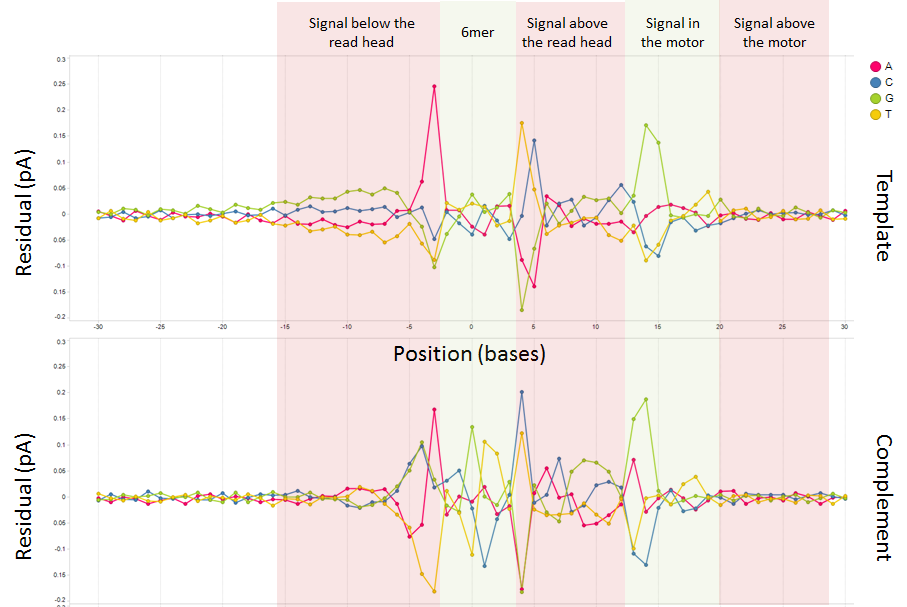
\includegraphics[width=\textwidth]{figures/context.png}
\caption[]{Long range signal context of the template strand. The median deviation of the model (y-axis) is plotted against the occurence of a certain nucleotide at a specific distance from the kmer (x-axis). The region from 0 to 6 refers to the actual 6-mer, which is taken into account by the model. }
\label{fig:context}
\end{figure}

As demonstrated in a Wiki-Post\footnote{\url{https://wiki.nanoporetech.com/display/DS/Spooky+action+at+a+distance+-+long+range+signal+context}} and in my \textit{IPython Notebooks} in \texttt{04\_error\_correction}, the 6-mer model does not model all information available from the data. Additional signals are detected about \SI{15}{nt} downstream, e.g. the abundance of Guanine at positions +14 and +15 tend to lead to a higher current level for a given 6-mer in the pore. (see figure \ref{fig:context}).

This information cannot be modeled using a HMM, as it requires information about nucleotides which are \textit{downstream}, i.e.\ not called yet. As a workaround I tried an iterative basecalling model (illustrated in fig. \ref{fig:iterative}): 

\begin{enumerate}
\item The HMM predicts the sequence from a given squiggle space as usual.
\item An SVM corrects the squiggle data given the predicted sequence. \label{itm:correct-squiggle}
\item The HMM re-predicts the sequence from the corrected squiggle space. 
\item continue with step \ref{itm:correct-squiggle} until satisfied. 
\end{enumerate}

\subsection{training of the SVM}
The training dataset was constructed from sequences successfully aligned to a reference genome with squiggle data available. For each position in the reference genome, I took only the \textit{median deviation from the model} ($\mathrm{mean}_\mathrm{kmer} - \mathrm{mean}_\mathrm{model}$) to avoid a bias towards regions with higher coverage. The mean, stdv and the nucleotides \num{+-20} around the 6-kmer were used as features. I encoded nucleotides as binary vector, i.e. $A=[1, 0, 0, 0], C=[0, 1, 0, 0]$ and so on. I used the \textit{median deviation from the model} as target value. The SVM achieved a pearson correlation coefficient (PCC) of 0.46 and a mean absolute error (MAE) of 0.62 in a 3-fold cross validation. For comparison: The mean \textit{median deviation from the model} over all genomic positions is 0.71. 

\subsection{result}
This approach lead to a significant increase in computation time, but did not improve the results (result not shown). This can either indicate insufficient performance of the SVM or the infeasibility of the entire approach. 


\begin{figure}[htbp]
\centering
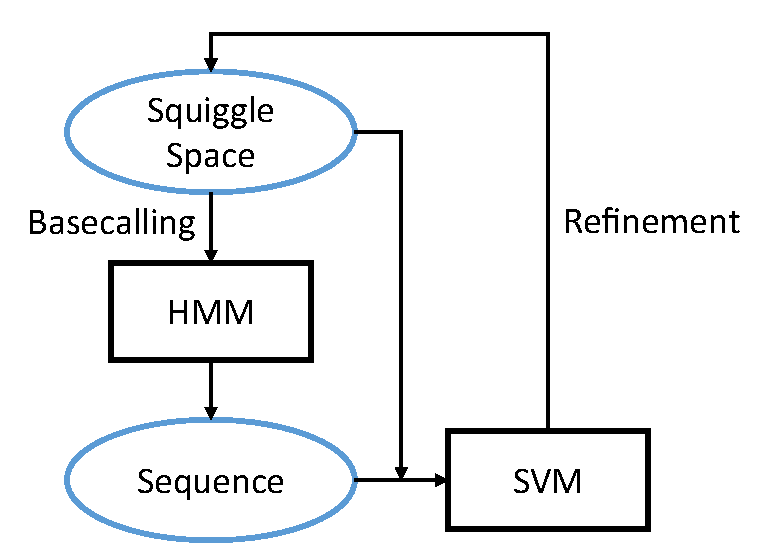
\includegraphics[width=.5\textwidth]{figures/iterative-basecalling.pdf}
\caption{Architecture of the iterative base-calling approach}
\label{fig:iterative}
\end{figure}
% explain the machine learning and document that there is a corresponding ipynb. 

\section{Future development}
\label{sec:future}
The nanopore sequencing is under very rapid development. Since the completion of this project, Oxford Nanopore has announced an open source version of their original Basecaller, developed a new generation of flow cells and a new kind of basecaller which is not based on HMMs any more and will also be released in an open source version. 
For more Information I recommend watching the Hangout by Oxford Nanopore CTO Clive Brown.\footnote{Available in the Nanoporetech wiki \url{https://wiki.nanoporetech.com/x/iD00Ag}}

\printbibliography


\end{document}
